\documentclass[12pt]{article}
%% arXiv paper template by Flip Tanedo
%% last updated: Dec 2016



%%%%%%%%%%%%%%%%%%%%%%%%%%%%%
%%%  THE USUAL PACKAGES  %%%%
%%%%%%%%%%%%%%%%%%%%%%%%%%%%%

\usepackage{amsmath}
\usepackage{amssymb}
\usepackage{amsfonts}
\usepackage{graphicx}
\usepackage{xcolor}
\usepackage{nopageno}
\usepackage{enumerate}
\usepackage{parskip}
\usepackage{framed}


\renewcommand{\thesection}{}
\renewcommand{\thesubsection}{\arabic{subsection}}

%%%%%%%%%%%%%%%%%%%%%%%%%%%%%%%%%%%%%%%%%%%%%%%
%%%  PAGE FORMATTING and (RE)NEW COMMANDS  %%%%
%%%%%%%%%%%%%%%%%%%%%%%%%%%%%%%%%%%%%%%%%%%%%%%

\usepackage[margin=2cm]{geometry}   % reasonable margins

\graphicspath{{figures/}}	        % set directory for figures

% for capitalized things
\newcommand{\acro}[1]{\textsc{\MakeLowercase{#1}}}    

%\numberwithin{equation}{section}    % set equation numbering
\renewcommand{\tilde}{\widetilde}   % tilde over characters
\renewcommand{\vec}[1]{\mathbf{#1}} % vectors are boldface

\newcommand{\dbar}{d\mkern-6mu\mathchar'26}    % for d/2pi
\newcommand{\ket}[1]{\left|#1\right\rangle}    % <#1|
\newcommand{\bra}[1]{\left\langle#1\right|}    % |#1>
\newcommand{\Xmark}{\text{\sffamily X}}        % cross out

\let\olditemize\itemize
\renewcommand{\itemize}{
  \olditemize
  \setlength{\itemsep}{1pt}
  \setlength{\parskip}{0pt}
  \setlength{\parsep}{0pt}
}


% Commands for temporary comments
\newcommand{\comment}[2]{\textcolor{red}{[\textbf{#1} #2]}}
\newcommand{\flip}[1]{{\color{red} [\textbf{Flip}: {#1}]}}
\newcommand{\email}[1]{\texttt{\href{mailto:#1}{#1}}}

\newenvironment{institutions}[1][2em]{\begin{list}{}{\setlength\leftmargin{#1}\setlength\rightmargin{#1}}\item[]}{\end{list}}


\usepackage{fancyhdr}		% to put preprint number



% Commands for listings package
%\usepackage{listings}      % \begin{lstlisting}, for code
%
% \lstset{basicstyle=\ttfamily\footnotesize,breaklines=true}
%    sets style to small true-type



%%%%%%%%%%%%%%%%%%%
%%%  HYPERREF  %%%%
%%%%%%%%%%%%%%%%%%%

%% This package has to be at the end; can lead to conflicts
\usepackage{microtype}
\usepackage[
	colorlinks=true,
	citecolor=black,
	linkcolor=black,
	urlcolor=green!50!black,
	hypertexnames=false]{hyperref}





\begin{document}


\begin{center}

    {\Large \textsc{Weekly HW 2}:
    \textbf{Indices. Indices everywhere.}}
    
\end{center}

\vskip .4cm

\noindent
\begin{tabular*}{\textwidth}{rl}
	\textsc{Course:}& Physics 165, \emph{Introduction to Particle Physics} (2018)
	\\
	\textsc{Instructor:}& Prof. Flip Tanedo (\email{flip.tanedo@ucr.edu})
	\\
	\textsc{Due by:}& {Tuesday}, January 23
\end{tabular*}

\noindent
This is the main weekly homework set. Unless otherwise stated, give all responses in natural units where $c = \hbar = 1$ and energy is measured in electron volts (usually MeV or GeV). 

\subsection{Momentum In a Loop}

Here's a diagram for a higher-order correction to $e^+ e^- \to Z$. 
\begin{center}
	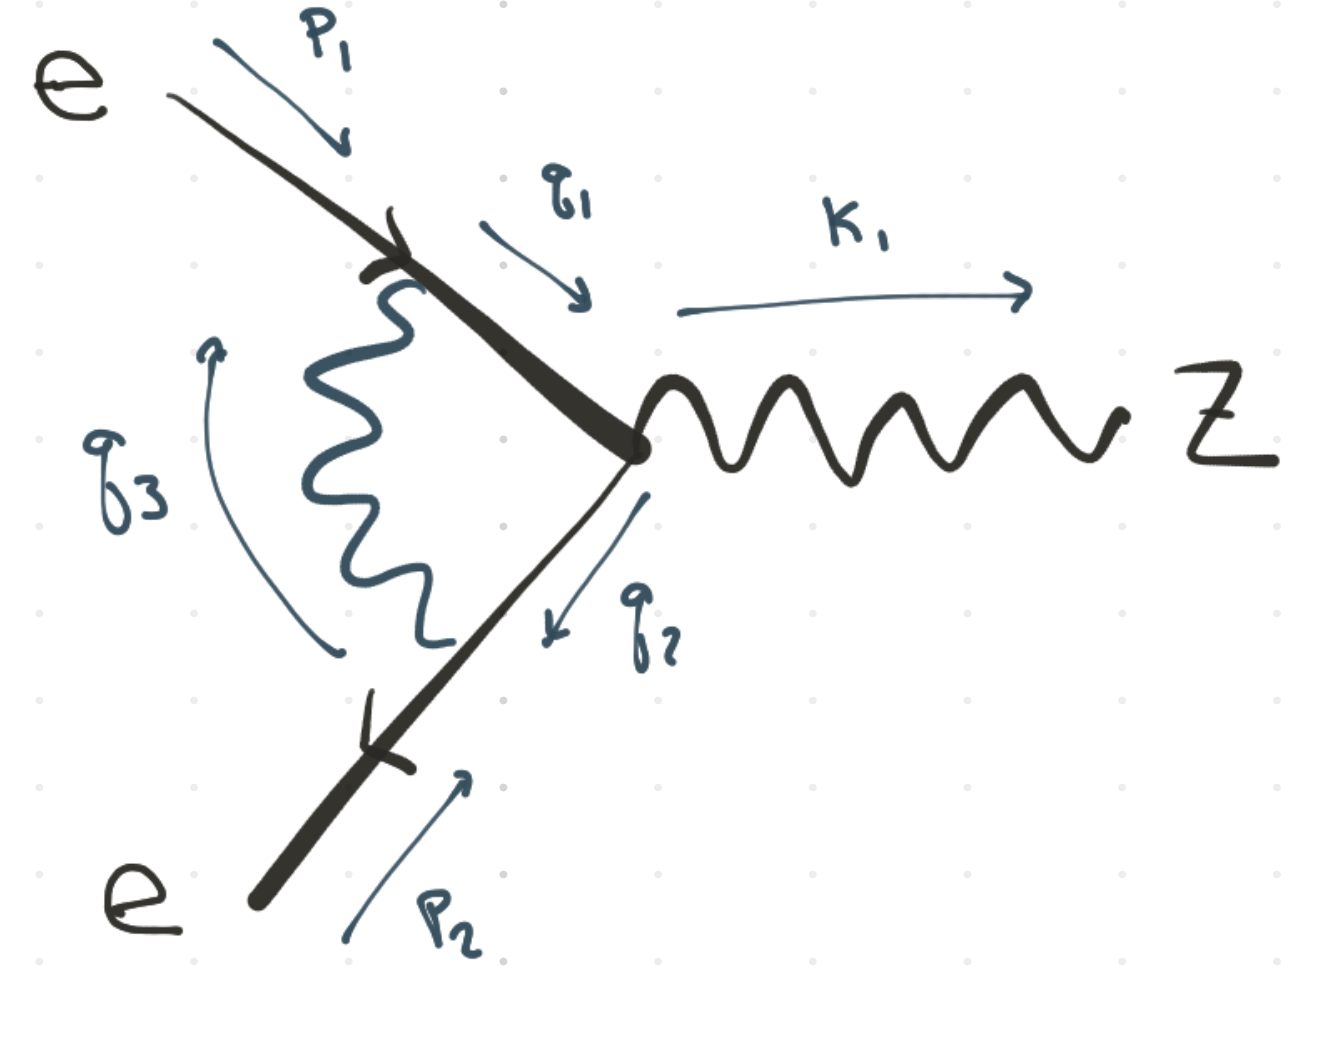
\includegraphics[width=.4\textwidth]{HW2b.png}
\end{center}

\subsubsection{What are the internal lines?}

In the diagram above, what are the possible particle species of the internal lines? Label them. Choose from $e,\mu, \nu_e, \nu_\mu, \gamma, Z$. 

\subsubsection{In-state/out-state kinematics}

In the center of mass frame for the system (the rest frame of the $Z$), what condition must be satisfied by the electron and positron momenta for this process to be kinematically possible? Now write this in terms of an \emph{invariant} quantity of the $e^+e^-$ system, so that you can specify a condition which must be true in \emph{any} frame.

\textsc{Discussion}: The remarkable observation about this process is that it looks like you need to tune your electron--positron energies to be \emph{exactly} the right in order to produce the $Z$ boson on-shell. This is in contrast to $e^+e^- \to \mu^+ \mu^-$, where as long as you have enough energy, you can produce the muons. If your $e^+e^-$ system has a little extra energy, then the muons are a little more energetic. In $e^+e^- \to Z$, if you give your $e^+e^-$ system a little extra energy, then you cannot produce the $Z$ on-shell. We will see that there's a little more to this story than we're presenting.

\subsubsection{Loop momentum}

Use conservation of four-momentum at each vertex to determine $q_1^\mu$, $q_2^\mu$ and $q_3^\mu$ in terms of the observed four-momenta, $p_1^\mu$, $p_2^\mu$, and $k_1^\mu$. 

\subsubsection{That's weird...}

In the previous sub-problem, you should find that you cannot determine $q_{1,2,3}$ uniquely. What do you think this means in terms of the sum of amplitudes? Think about it this way: each possible assignment of momentum flow is a possible history between the $|\text{ in }\rangle$ and the $|\text{ out }\rangle$ states. Answer in a few sentences. 

\textsc{Comment}: There's no strict criteria for what you must answer, but I'd like you to think about this and convey (i) understanding of the situation and (ii) thoughts/speculation about interpretation.



\subsection{Indices and what they tell us}

The ``index-ology'' that we're proposing has a high-brow name: the representation theory of Lie groups. We will use the Define the \textbf{Einstein summation convention}:
\begin{quote}
	Repeated indices are summed over. 
\end{quote}
 There's no physics and no mathematics in this, it's simply a shorthand to avoid writing the sum symbol. \emph{Most of the time} we require that one of the repeated indices is upper and the other is lower. In this problem that is indeed the case. Thus, for example:
 \begin{align}
 	T^{ij}y_j \equiv \sum_j T^{ij}y_j = T^{i1}j_1 + T^{i2}j_2 + \cdots \ .
 \end{align}
 This object has one \textbf{free index}, $i$, because the $j$ index is repeated and hence summed over. In other words: in order to get a \emph{number}, I have to specify what $i$ is. 


\subsubsection{Rotations: SO(2)}

SO(2) is the fancy name for rotations in two-dimensional space. Let's introduce two kinds of objects that transform under rotations: \textbf{column vectors}, $v^i$, and \textbf{row vectors}, $w_j$.% You could also call these $\vec{v}$ and $\vec{w}^T$.

\begin{framed}
\textsc{Caveats!} I am now guilty of propagating some terrible misunderstandings that is unfortunately rife among physics students. Here are some of them:
\begin{enumerate}
	\item There are many words for the objects that I'm calling column and row vectors. The words that we're using should be the most familiar, but it's also the notation that mathematicians use for their kindergarten-age children. If you're ever in a cocktail party with mathematicians, then you might want to say things like covariant/contravariant, or vector/one-form, or vector/dual vector. These sound way fancier, but for our immediate purposes do not convey any deeper meaning. 
	\item Much worse, I'm voluntarily committing the cardinal sin of using the \emph{components} of an object to represent the object itself. I'm assuming that we have all agreed upon the right basis $\vec{e}_{(1)}$ and $\vec{e}_{(2)}$, so that writing $v^i$ can mean either vector $$\vec{v} = v^1 \vec{e}_{(1)} + v^2 \vec{e}_{(2)},$$ or the $i^\text{th}$ component of that vector, that is $v^1$ for $i=1$ or $v^2$ for $i=2$. The basis vectors are abstract objects and don't have to represent anything; but they could be, for example, any of the following:
\begin{align}
	\vec{e}_{(1)} & = \begin{pmatrix}1\\0\end{pmatrix}
	&
	\vec{e}_{(2)} & = \begin{pmatrix}0\\1\end{pmatrix}
	\\
	\vec{e}_{(1)} & = \frac{1}{\sqrt{2}}\begin{pmatrix}0\\1\\1\end{pmatrix}
	&
	\vec{e}_{(2)} & = \frac{1}{\sqrt{2}}\begin{pmatrix}0\\1\\-1\end{pmatrix}
	\\
	\vec{e}_{(1)} & = \left|\text{ cat alive } \right\rangle
	&
	\vec{e}_{(2)} & = \left|\text{ cat dead } \right\rangle
\end{align}
or any other orthonormal set of objects. The point is that we've agreed upon what they are (or agreed to not worry about it) and that we'll focus on the components $v^1$ and $v^2$.
\end{enumerate}
\end{framed}
Here are the rules for upper and lower indices:
\begin{enumerate}
	\item Each upper index transforms with a rotation matrix, $R^i_{\phantom i j}$. 
	\item Each lower index transforms with a rotation matrix in the opposite direction, $(R^{-1})^i_{\phantom i j}$. 
\end{enumerate}
thus we have the transformation rules that under a rotation by $\theta$,
\begin{align}
	v^i &\to (v')^i = R^i_{\phantom i j} v^j = R^i_{\phantom i 1}v^1 + R^i_{\phantom i 2}v^2
	\label{eq:v}
	\\
	w_j &\to (w')_j = (R^{-1})^i_{\phantom i j} w_i = (R^{-1})^1_{\phantom 1 j}w_1 + (R^{-1})^2_{\phantom 2 j}w_2 \ .
	\label{eq:w}
\end{align}
The components of a rotation are:
\begin{align}
	R^1_{\phantom 1 1} &= \cos \theta
	&
	R^1_{\phantom 1 2} &= \sin\theta
	&
	R^2_{\phantom 2 1} &= -\sin\theta
	&
	R^2_{\phantom 2 2} &= \cos \theta 
	\label{eq:rot}
	\\
	(R^{-1})^1_{\phantom 1 1} &= \cos \theta
	&
	(R^{-1})^1_{\phantom 1 2} &= -\sin\theta
	&
	(R^{-1})^2_{\phantom 2 1} &= \sin\theta
	&
	(R^{-1})^2_{\phantom 2 2} &= \cos \theta \ .
\end{align}

Explicitly write the components $(v')^i$ and $(w')_j$ in terms of the components $v^i$ and $w_j$. For example, the first one is:
\begin{align}
	(v')^1 = \cos \theta \, v^1 + \sin\theta  \, v^2 \ .
\end{align}
Confirm that this is indeed the same thing as ordinary matrix multiplication,
\begin{align}
\vec{v}' &=
 \begin{pmatrix}
		\cos \theta & \sin \theta \\
		-\sin \theta & \cos \theta
	\end{pmatrix}
	\begin{pmatrix}
		v^1 \\
		v^2
	\end{pmatrix} 
	&
\vec{w'}^T &=
\left[
 \begin{pmatrix}
		\cos \theta & \sin \theta \\
		-\sin \theta & \cos \theta
	\end{pmatrix}
	\begin{pmatrix}
		w^1 \\
		w^2
	\end{pmatrix} \right]^T
	\ .
\end{align}

\textsc{Remark}: yes, you \emph{know} what the answer is---do it usng the sums in (\ref{eq:v}) and (\ref{eq:w}) so that you see how the notation works.

\subsubsection{How matrices transform} 

The object that you know of as a `matrix' has one upper and one lower index. Each index transforms according to the rules above:
\begin{align}
	M^i_{\phantom i j} 
	\to (M')^i_{\phantom{i} j} 
	= (R^{-1})^k_{\phantom{k} j} R^i_{\phantom{i}\ell} M^\ell_{\phantom\ell k} \ .
\end{align}
Confirm that this is equivalent to the `usual' rule
\begin{align}
	\begin{pmatrix}
		m^1_{\phantom 1 1} & m^1_{\phantom 1 2}
		\\
		m^2_{\phantom 2 1} & m^2_{\phantom 2 2}
	\end{pmatrix}
	\to 
	\begin{pmatrix}
		\cos \theta & \sin \theta \\
		-\sin \theta & \cos \theta
	\end{pmatrix}^T
	\begin{pmatrix}
		m^1_{\phantom 1 1} & m^1_{\phantom 1 2}
		\\
		m^2_{\phantom 2 1} & m^2_{\phantom 2 2}
	\end{pmatrix}
	\begin{pmatrix}
		\cos \theta & \sin \theta \\
		-\sin \theta & \cos \theta
	\end{pmatrix} \ .
\end{align}

\textsc{Remark}: Observe that unlike the usual matrix multiplation where the order of the matrices matter, 
\begin{align*}
(R^{-1})^k_{\phantom{k} j} R^i_{\phantom{i}\ell} M^\ell_{\phantom\ell k}
=
(R^{-1})^k_{\phantom{k} j}  M^\ell_{\phantom\ell k}	R^i_{\phantom{i}\ell}
=
R^i_{\phantom{i}\ell}  M^\ell_{\phantom\ell k} (R^{-1})^k_{\phantom{k} j}
= \cdots
\end{align*}
This is because the summation convention is taking care of the  kindergarten matrix multiplication rule that one should `tip the matrix over and then sum the pieces that hit the next matrix.' More importantly, this lets us generalize that rule to the case of objects with many indices. 

\subsubsection{An SO(2) invariant} 

We say that objects with indices are \textbf{covariant}, they change in a specific way with respect to rotations. This is in contrast to objects with no indices, which are \textbf{invariant} or \textbf{scalar}. 

Because $v^i$ has an upper index an $w_j$ has a lower index, you can \textbf{contract} them to form an object with no indices:
\begin{align}
	v^i w_i \equiv v^1 w_1 + v^2 w_2  \ .
\end{align}

Confirm that this object---which you know as the usual dot product---is indeed invariant by calculating $(v')^i(w')_i$. 

\subsubsection{The metric on flat two-dimensional space} 

We can introduce an additional mathematical structure to our vector space: a \textbf{metric}. This is an object that lets us raise and lower indices. In 2D flat space, we know this operation as \textbf{transpose}. More generally, it is the Kronecker $\delta$:
\begin{align}
	\delta_{ij} &=
	\left\{
	\begin{array}{lcl}
		1 & \quad & \text{if $i = j$}\\
		0 & \quad & \text{otherwise}
	\end{array}
	\right.
	&
	\delta^{ij} &=
	\left\{
	\begin{array}{lcl}
		1 & \quad & \text{if $i = j$}\\
		0 & \quad & \text{otherwise}
	\end{array}
	\right.
\end{align}
Thus we may write
\begin{align}
	v\cdot v = v^i v_i = v^i (\delta_{k i} v^k) \ ,
\end{align}
where in the last equation we have used the $\delta_{ki}$ to create a lower-index object $v_i$ out of an upper-index object, $v^k$. This lets us define a \textbf{norm} of a vector:
\begin{align}
	|\vec v| = \sqrt{v\cdot v} \equiv \sqrt{ \delta_{k i} v^iv^k} \ .
\end{align}
Confirm the trivial statement that the lower-index $\delta_{ij}$ is the \emph{inverse} of the upper-index $\delta^{ij}$. In other words, confirm that
\begin{align}
	\delta_{ik}\delta^{kj} = \delta_i^j &=
	\left\{
	\begin{array}{lcl}
		1 & \quad & \text{if $i = j$}\\
		0 & \quad & \text{otherwise}
	\end{array}
	\right. \ .
\end{align}

\subsubsection{Boosts: SO(1,1)}

SO(1,1) is the fancy name for Lorentz transformations in two-dimensional space\emph{time}. To distinguish from just space, we will use lowercase Greek letters like $\mu$. These will take values starting at $\mu = 0$ to denote the time component. The rules for upper and lower indices are the same, so that 
\begin{align}
	p_\mu x^\mu = p_0 x^0 + p_1 x^1 \ .
\end{align}
There are no minus signs yet! Similarly, objects transform according to a `rotation' in spacetime that we call a \textbf{Lorentz transformation},
\begin{align}
	\Lambda^\mu_{\phantom \mu \nu} &= 
	\begin{pmatrix}
		\gamma & \gamma \beta
		\\
		\gamma \beta & \gamma
	\end{pmatrix}
	&
	\gamma = \frac{1}{\sqrt{1-\beta^2}} \ .
	\label{eq:boost}
\end{align}
The sign of $\beta$ depends on whether you're defining an active versus a passive transformation in the same way that the sign of $\theta$ is similarly ambiguous for rotations.

The key difference between space\emph{time} and space is a crucial minus sign in the \textbf{metric}, which we now write as $\eta$:
\begin{align}
	\eta_{\mu\nu} &= \begin{pmatrix}
		-1 & 0 \\
		0 & 1
	\end{pmatrix}
	&
	\eta^{\mu\nu} &= \begin{pmatrix}
		-1 & 0 \\
		0 & 1
	\end{pmatrix} \ .
\end{align}
Confirm that $\eta_{\mu\nu} \eta^{\nu\sigma} = \delta^\sigma_\mu$.


\subsubsection{Spacetime invariant}

Momenta typically have lower indices, $p_\mu$. This is because they inherit the index structure from derivatives, $\partial_\mu = \partial/\partial x^\mu \to -i p_\mu $, which you may remember from quantum mechanics. (I'm guessing on the sign.) When we do kinematics, it is common for many references to assume that momenta `naturally' come with upper indices, $p^\mu$. For the most part this is fine as long as one is consistent. For the rest of this problem we'll assume the upper index, so that
\begin{align}
	p^\mu &= (p^0, p^1) 
	&
	p^0 &= E 
	&
	p^1 &= p \ .
\end{align}
Write out $p\cdot p = p^\mu p_\mu$ and confirm that it is invariant under Lorentz transformations. Recall the on-shell relation and confirm that a convenient name for this invariant is $p\cdot p = m^2$.

\subsubsection{Rotations in spacetime}

You may remember (\ref{eq:boost}) from an introduction to special relativity. $\beta$ is the velocity in natural units, $\beta = v/c$. $\gamma$ is often called the \textbf{boost} factor, it's larger than 1 and tells you about length contraction and time dilation. Mathematically, though, (\ref{eq:boost}) is kind of a funny form. Recall that on flat \emph{space}, the norm of a vector is invariant under rotations. This made sense because the rotations were written with respect to trigonometric functions, and we knew that $\sin^2\theta + \cos^2\theta = 1$. For Minkowski space, which is what math-y people call flat spacetime, the analog for this are the hyperbolic trigonometric functions, which satisfy
\begin{align}
	\cosh^2 w - \sinh^2 w = 1 \ . 
\end{align}
In fact, a Lorentz transformation can equivalently be written
\begin{align}
		\Lambda^\mu_{\phantom \mu \nu} &= 
	\begin{pmatrix}
		\cosh w & \sinh w
		\\
		\sinh w & \cosh w
	\end{pmatrix}
\ .
\end{align}
Confirm that this is consistent with (\ref{eq:boost}):
\begin{enumerate}
	\item If you identify $\cosh w = \gamma$ and $\sinh w = \gamma\beta$, confirm that the hyperbolic identity holds $\cosh^2 w - \sinh^2 w = 1$.
	\item Explicitly derive $w$ as a function of $\beta$.
\end{enumerate}
The parameter $w$ is called the \textbf{rapidity}.

\subsubsection{Rotations/Boosts as a group}

Write the rotation in (\ref{eq:rot}) as $R(\theta)$. Confirm that $R(\theta_1)R(\theta_2) = R(\theta_1+\theta_2)$. That is:
\begin{align}
	R(\theta_1)^i_{\phantom i k}
	R(\theta_2)^k_{\phantom k j} 
	= R(\theta_1+\theta_2)^i_{\phantom i j} \ .
\end{align}
Do the same for boosts, confirm that $\Lambda(w_1)\Lambda(w_2) = \Lambda(w_1+w_2)$, or:
\begin{align}
	\Lambda(w_1)^\mu_{\phantom \mu \sigma}
	\Lambda(w_2)^\sigma_{\phantom \sigma \nu} 
	= \Lambda(w_1+w_2)^\mu_{\phantom \mu \nu} \ .
\end{align}
\textsc{Remark}: If you are familiar with group/representation theory, you may be nodding along. If you are not, then don't sweat it. You're not missing anything. Groups are mathematical constructs for which relations like these are true. Technically all that we're saying is that two consecutive rotations are also a rotation. This sounds trivial---and indeed, based on everything we know about rotations it is---but it's not true for other classes of matrices. For example, the class of $2\times 2$ matrices with the upper right component is $3$ does not form a group because applying to such matrices consecutively does not always produce a matrix whose upper right component is $3$.





\subsection{$\mu \to e \gamma$, again}

Quite the contrary to last week's erroneous homework problem, go ahead and draw a leading-order Feynman diagram for $\mu \to e \gamma$. You'll need to use the the $W$ boson:
\begin{center}
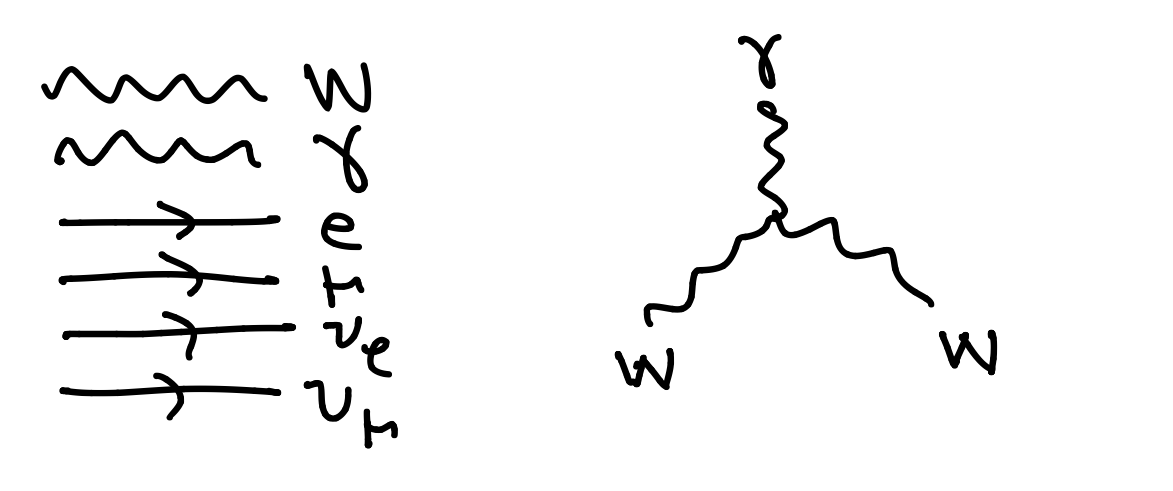
\includegraphics[width=.5\textwidth]{HW2bbbb.png}
\end{center}
The $W$ boson is an electrically charged particle, thus it has an antiparticle that is conventionally drawn the same way\footnote{You could draw electric charge arrows on the $W$, but we don't do this... eventually there are too many charges to keep track of. Convince yourself that there's no ambiguity.}. The $W$ couples to the electron, muon, electron-neutrino, and muon-neutrinos as follows:
\begin{center}
	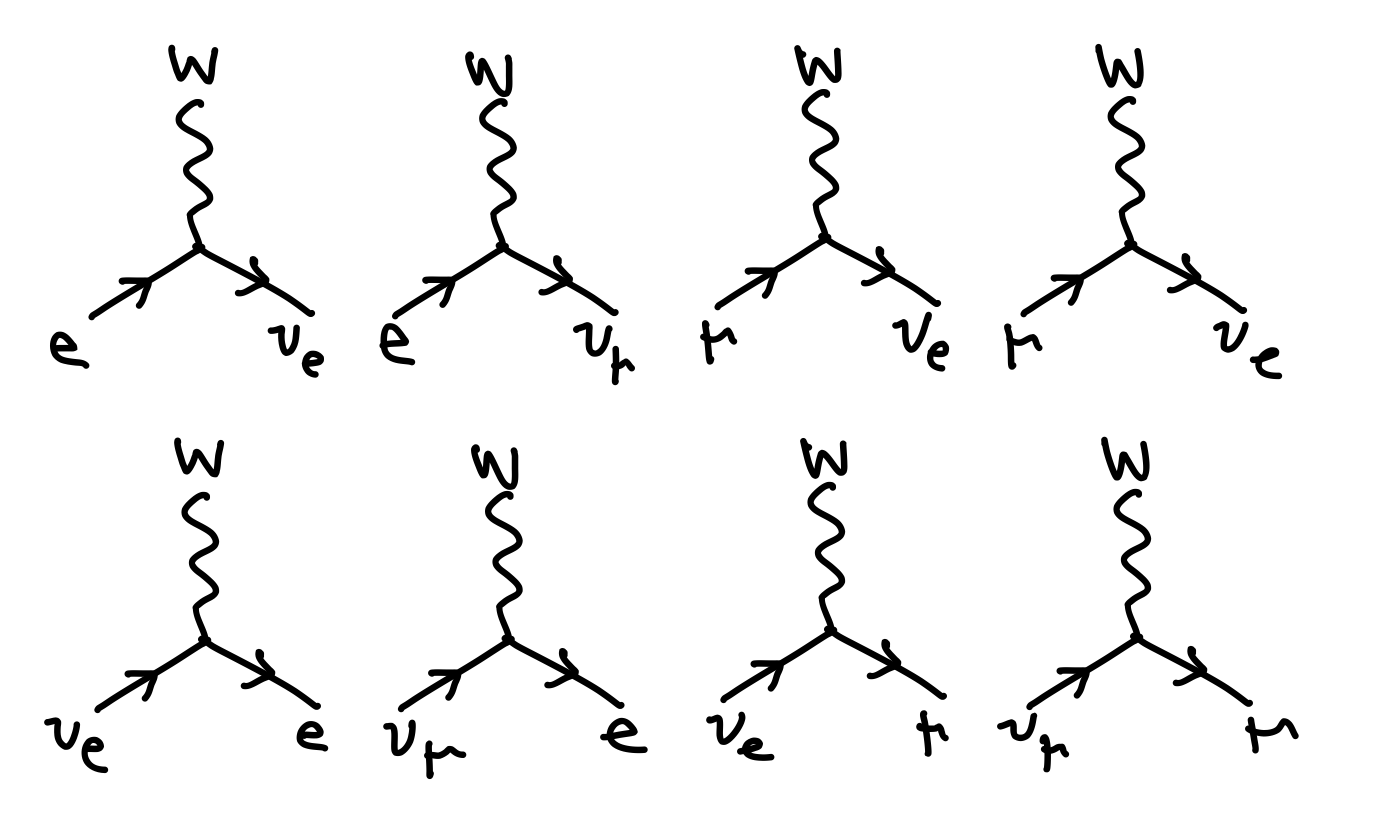
\includegraphics[width=.8\textwidth]{HW2bb.png}
\end{center}
Note that electric charge is conserved in these interactions.



You should be able to draw a diagram for $\mu \to e \gamma$. It won't be a simple one! The topology will look familiar. Comment on conservation laws. Why could you \emph{not} draw this diagram in QED---what conservation law prevented it? How do the $W$ Feynman rules break these conservation laws? 

\textsc{Remark}: Technically the rules drawn here are not part of the Standard Model, but they are closer to reality. (These rule implicitly assume the existence of neutrino mass.)



\subsection{Feedback}

Approximately how long did it take you to complete the non-extra credit parts of this assignment?




\section{Extra Credit}

If you do any of these problems, please write a short note giving your thoughts on the reading: did you like them? Were they too simple / difficult? I do not expect you to be able to complete all (or necessarily any) of the extra credit.

\subsection{Direct Detection of Dark Matter}

This is an exercise in non-relativistic kinematics. One way to search for dark matter is to wait for it to hit a xenon nucleus and detect the recoil of the nucleus. In this problem, we use the `sum over all possible paths' mantra of quantum mechanics to explain why we use xenon as opposed to something cheaper, like helium. 

For simplicity, assume that both the mass of the dark matter and the mass of the xenon nucleus is $m_{\text{DM}} = m_{\text{Xe}}=100~$GeV. Assume that in the \textbf{lab frame}, the xenon nucleus is at rest and that the dark matter particle is traveling at $(v_\text{DM}^\text{lab})=300~$km/s. You can work to one significant figure in this problem (you may want to keep 2 significant figures for intermediate steps). 

\subsubsection{Momentum transfer}
The transfer 3-momentum, $\vec q$, is the 3-momentum that the incident dark matter particle imparts on the nucleus at rest. Everything is happening slowly enough that special relativity doesn't affect anything, so we can add velocities in the simple (Galilean) way. Derive the expression for the magnitude transfer momentum, 
\begin{align}
	|\vec q|^2 = 2\mu^2 (v_\text{DM}^\text{lab})^2 (1\pm \cos \theta_\text{cm}) \ ,
\end{align}
where the sign of the angle depends on how it's defined. Here `cm' means `center of mass frame', $\mu = m_{\text{DM}}m_{\text{Xe}}/(m_{\text{DM}}+m_{\text{Xe}})$ is the dark matter--nucleus reduced mass. This is an exercise in Newtonian kinematics.


\subsubsection{de Broglie wavelength}

\emph{You can do this independently of the previous part.} 

Estimate the magnitude of the momentum transfer,
\begin{align}
	|\vec q| \approx \mu (v_\text{DM}^\text{lab}) \ .
\end{align}
Recall that the \textbf{de Broglie wavelength} of a particle is $\lambda = 2\pi\hbar/|\vec q|$. Of course, $\hbar = 1$ in this class. What is the approximate de Broglie wavelength associated with the dark matter scattering off the nucleus?

This wavelength describes the length scale that the interaction is probing. The size of a `big' nucleus is around 10~fm. Confirm that the de Broglie wavelength encompasses a `big' nucleus.

\subsubsection{Coherent scattering}

We assume that dark matter interacts with the protons and neutrons in the nucleus. Protons and neutrons are collectively known as nucleons. We assume that the dark matter talks to all nucleons equally.
If the de Broglie wavelength is larger  than the size of the nucleus, then the dark matter particle `sees' all of nucleons in the nucleus. Thus if the dark matter scatters off the nucleus, the scattering is actually a sum over the amplitude for dark matter to scatter off of one of the protons, plus the amplitude for dark matter to scatter off of a different proton, plus the amplitude for dark matter to scatter off one of the neutrons, etc.

How much more \emph{likely} is it for dark matter to scatter off of a heavy nucleus with atomic mass number $A$ compared to a light nucleus like helium with atomic mass number 4? This is why we fill our detectors with liquid xenon rather than helium.




\end{document}